\documentclass{article}
\usepackage{tikz, comment}
\usepackage{pifont}
\usepackage{fontspec}
\usetikzlibrary{arrows, decorations.markings, decorations.pathreplacing}
\begin{comment}
:Title: Not defined yet
:Tags: area using polar coordinates, polar integral formula ;polar form of a complex number;polar coordinates;cardioid;arc length of a curve
:Prob: 0.4548;0.4179;0.3601;0.3595;0.3417
:Author: Prof.Hu Ji-shan, HKUST
:Slug: No name yet

Description Here.........
\end{comment}
\begin{document}\centering

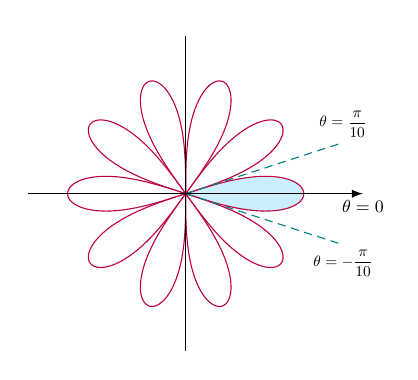
\begin{tikzpicture}[>=latex,xscale=.5*1, yscale=.5*1][font=\sf\small]

%\draw[xstep=1cm,ystep=1cm,color=gray!80] (0, -1) grid (8, 8);

\draw[purple, fill=cyan!20, samples=100, smooth, domain=-1*pi/10:1*pi/10, variable=\t]
plot ({3*sqrt(cos(5*\t r))*cos(\t r)}, {3*sqrt(cos(5*\t r))*sin(\t r)})--(0,0);

\foreach \n in {1,2,3,4,5,6,7,8,9}
{
\begin{scope}[rotate around={(\n)*36:({0}, {0})}]
\draw[purple, fill=white, samples=100, smooth, domain=-1*pi/10:1*pi/10, variable=\t]
plot ({3*sqrt(cos(5*\t r))*cos(\t r)}, {3*sqrt(cos(5*\t r))*sin(\t r)})--(0,0);

\end{scope}
};

\draw[densely dashed, teal, samples=100, smooth, domain=0:4, variable=\x]
plot ({\x}, {tan(pi/10 r)*(\x)})node[above, black, scale=0.6] {$\displaystyle \theta=\frac{\pi}{10}$};

\draw[densely dashed, teal, samples=100, smooth, domain=0:4, variable=\x]
plot ({\x}, {tan(-pi/10 r)*(\x)})node[below, black, scale=0.6] {$\displaystyle \theta=-\frac{\pi}{10}$};

\foreach \x in {}
\draw (\x,2pt/6) -- (\x,-2pt/6)
node[anchor=north] {\tiny$\x$}
;

\foreach \x in {}
\draw (\x,2pt/2.5) -- (\x,-2pt/2.5)
node[anchor=south] {\tiny$\x$}
;
\foreach \y in {}
\draw (-2pt/6,\y) -- (2pt/6,\y)
node[anchor=east] {\tiny $\y$}
;

\draw[->] (-4, 0) -- (4.5, 0)node[below, scale=0.7] {$\theta=0$} ;
\draw[] (0, -4) -- (0, 4)node[left] {};

%\node[yshift=0] at (-0.2/1, -0.2/1) {\tiny$0$};

\end{tikzpicture}
\end{document}